\chapter{Results}%Or Results
Let us start drawing a big picture of the different topics that emerged after the latent ideology analysis. 

For cop26 topic modeling found 70 topics, the first step in the analysis was to remove all the topics with less than 2000 users, after the first filtering the topics left are 46. 

After the latent ideology analysis some labels have been discarded because there were not enought edges to compute a statistically significative analysis. The final number of topics is 26.

 At this point for cop26 we have assigned a latent ideology score to 1557 influencers and 22161 users on 26 topics. 

The mean number of users with a ideology score for each topic is 1311, with a min of 151 and a max of 7764. Fig \ref{tab:recap_ideology} contains a reap of all this results for both COP26 and COP21

\begin{table}[h]
    \centering
    \begin{tabular}{|l|l|l|}
        \hline
        \textbf{Description} & \textbf{COP21} & \textbf{COP26} \\ \hline
        Initial topics & 36 & 70 \\ \hline
        Topics >2000 users & 18 & 46 \\ \hline
        Final topics & 4 & 26 \\ \hline
        Influencers scored & 270 & 1557 \\ \hline
        Users scored & 7931 & 22161 \\ \hline
        Mean users/topic &  2058 & 1311 \\ \hline
        Min users/topic & 35 & 151 \\ \hline
        Max users/topic & 7524 & 7764 \\ \hline
        \end{tabular}
        \caption{Summary of Latent ideology}
    \label{tab:recap_ideology}
\end{table}


\begin{figure}
    \centering
    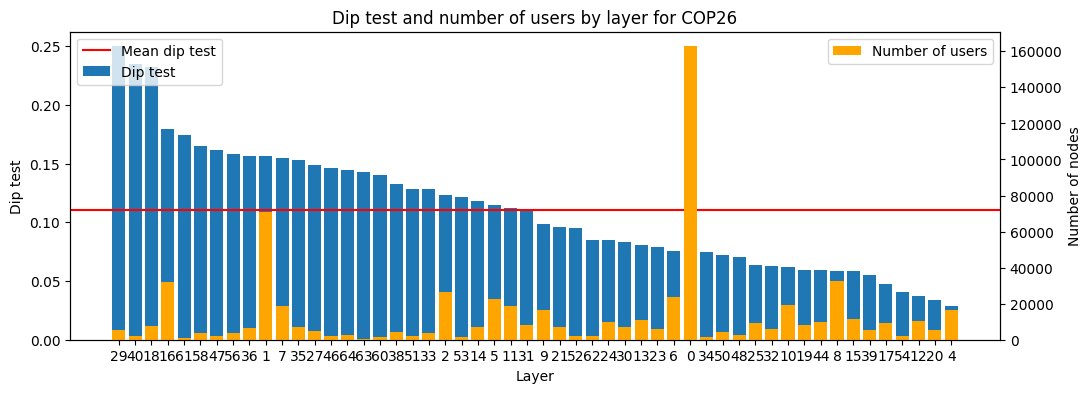
\includegraphics[width=0.95\linewidth]{Chapter5//figures/diptest_cop26.png}
    \caption{Dip test and number of users for the layer with at least 2000 nodes}
    \label{fig:diptest}
\end{figure}

\section{RQ1 Most Polarized Topics}

Fig \ref{fig:diptest} summarize the size and the diptest result, so the polarization, for each topic. The first thing to note is the fact that to the highest polarization corresponds the smaller topics, with the exception of topic 14. For the first to topics the polarization is significantly higher than the others.

Fig \ref{fig:networks_polarization} let us visualize the most and the least polarized topics, every network represent the retweet network of the 100 biggest influencers, in the leftmost plot we can find the full network while in the rightmost only the influencers are present. In the most polarized topics we can clearly see how the influencers are almost equally split between the two poles. The color of the node depends on its ideology score

It is interesting to note in Fig \ref{fig:ridge_topics} the distribution of the tweets of each topics over time during the cop, the dotted line marks the start end end date of COP26. The most polarized had interest only in few days losing quickly the interest. The opposite happens in the least polarized topics where the discussion is distributed over a longest timespan.  



\begin{figure}
    \centering
    \begin{minipage}{0.50\textwidth}
        \centering
         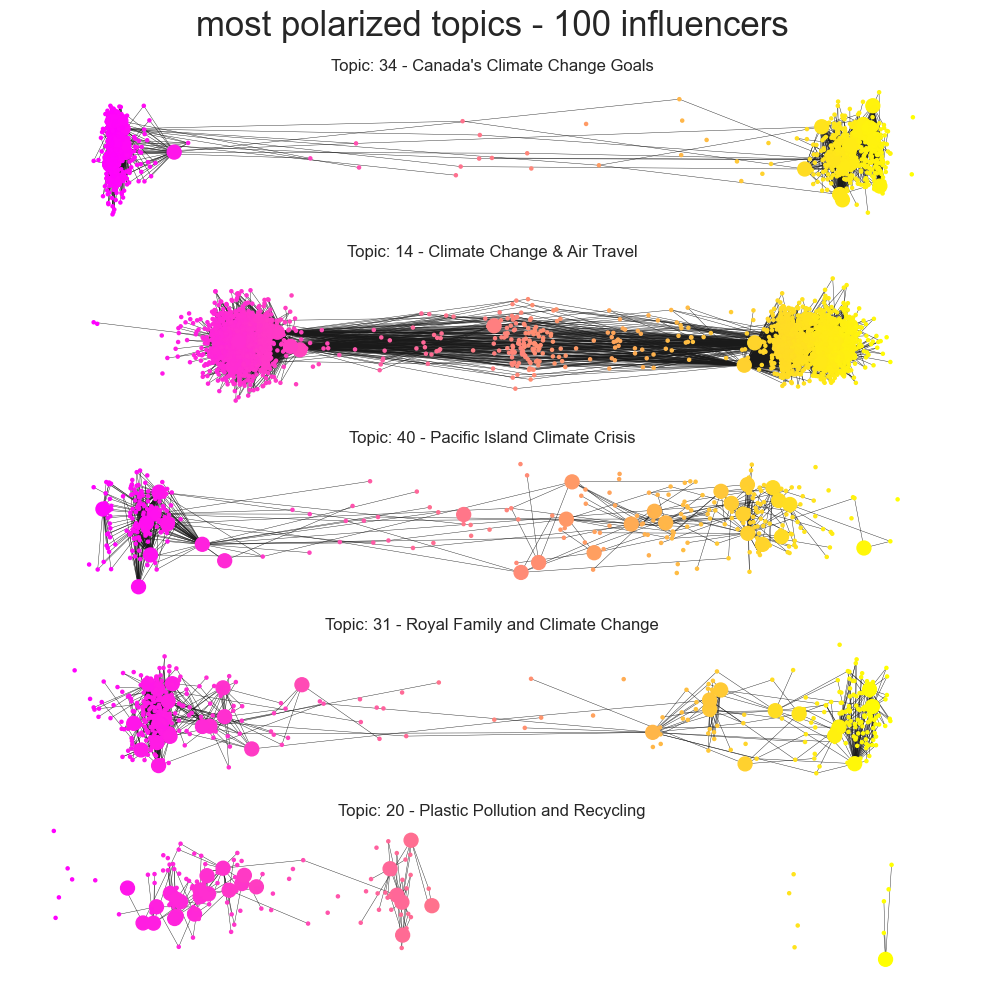
\includegraphics[width=0.98\linewidth]{Chapter5//figures/most_pol_cop26.png}
        \caption{most polarized topics}
    \end{minipage}\hfill
    \begin{minipage}{0.50\textwidth}
        \centering
         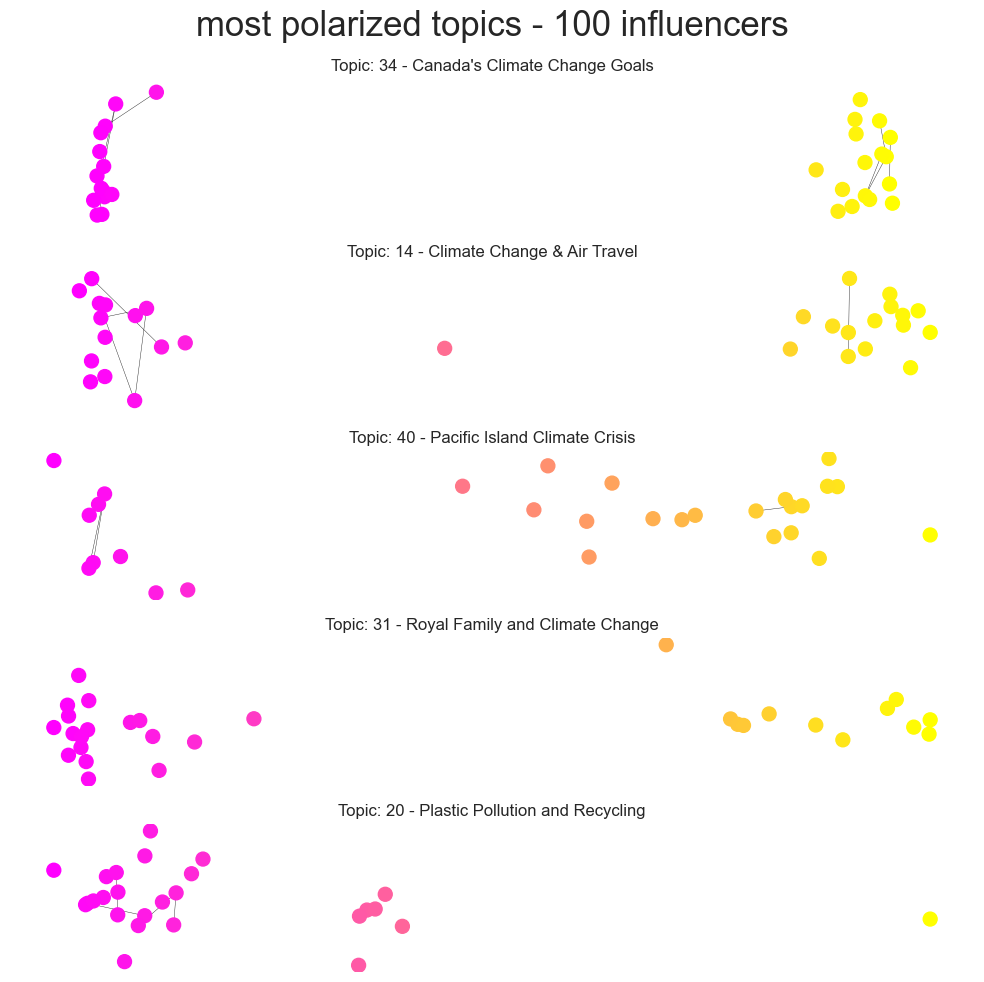
\includegraphics[width=0.98\linewidth]{Chapter5//figures/most_pol_cop26_inf.png}
        \caption{most polarized topics only infleuncers}
    \end{minipage}
    \begin{minipage}{0.50\textwidth}
        \centering
         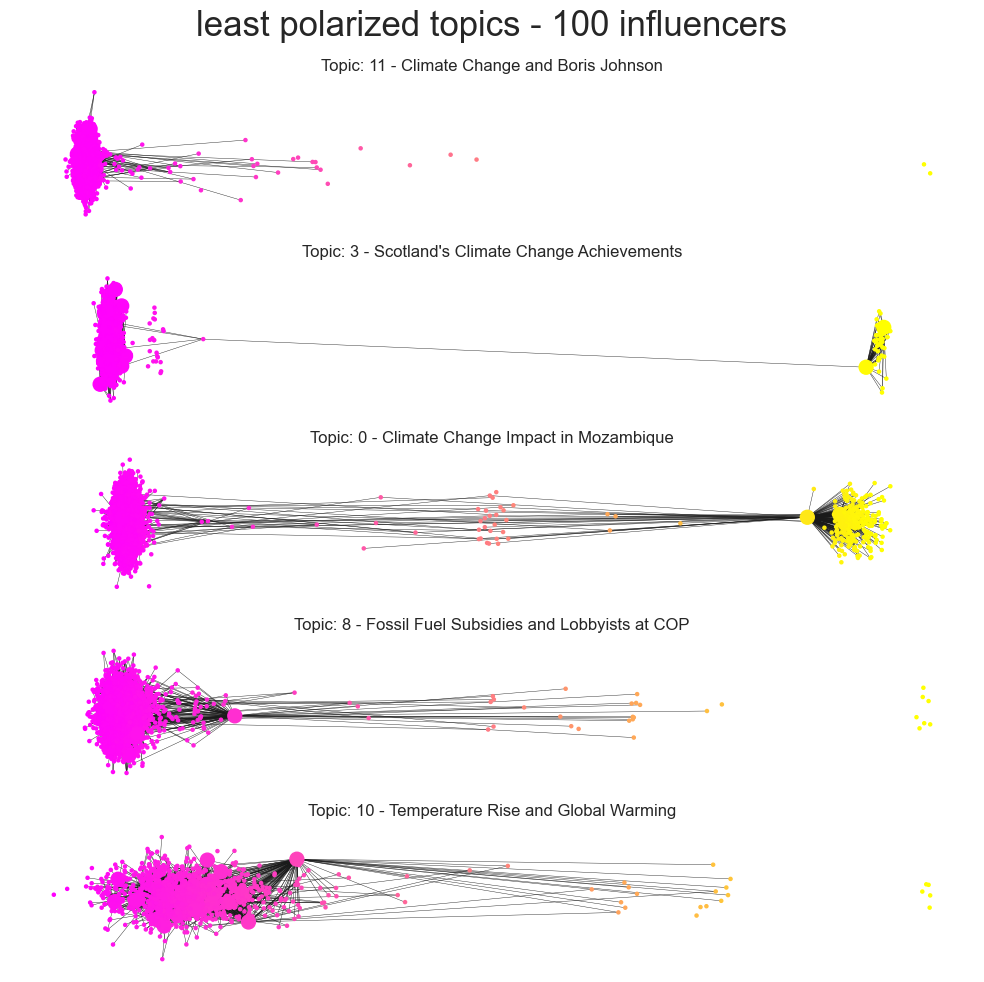
\includegraphics[width=0.98\linewidth]{Chapter5//figures/least_pol_cop26.png}
        \caption{least polarized topics}
    \end{minipage}\hfill
    \begin{minipage}{0.50\textwidth}
        \centering
         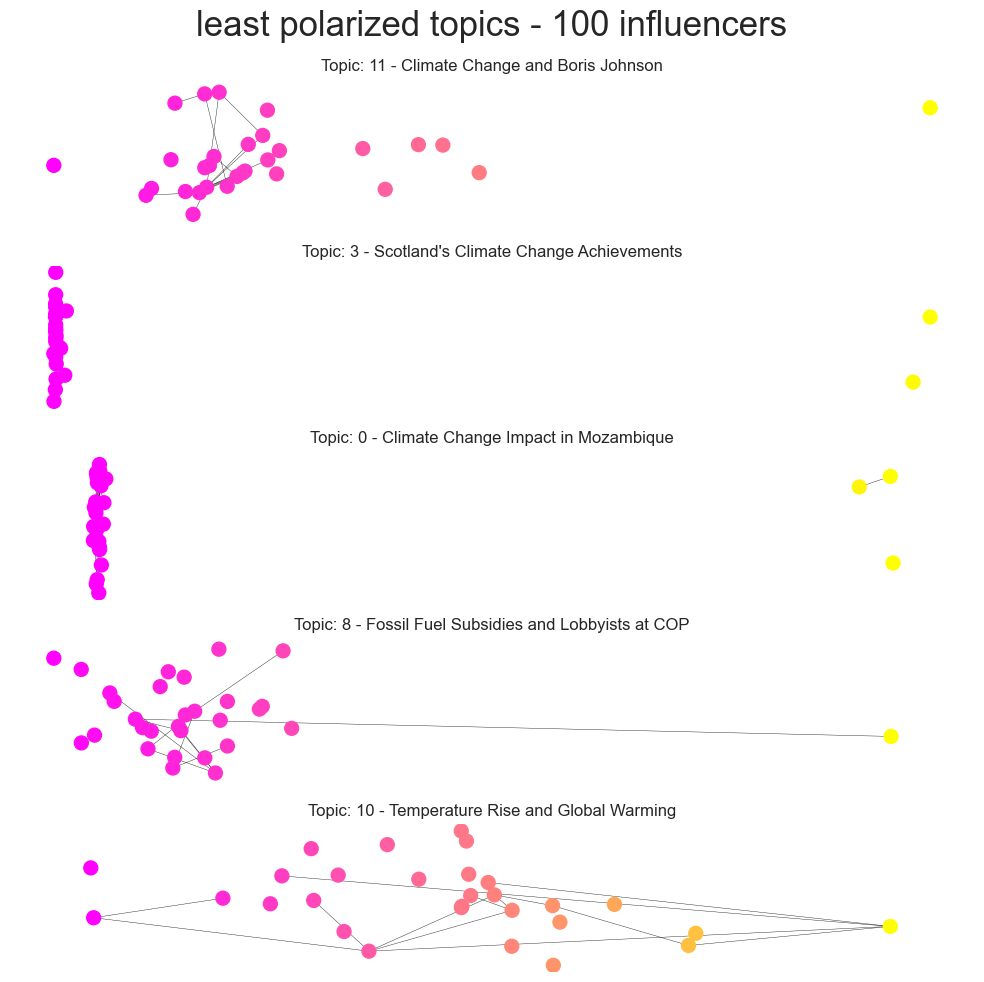
\includegraphics[width=0.98\linewidth]{Chapter5//figures/least_pol_cop26_inf.png}
        \caption{least polarized topics only influencers}
    \end{minipage}

    \caption{least and most polarized topics}
    \label{fig:networks_polarization}
\end{figure}


\begin{figure}
    \centering
    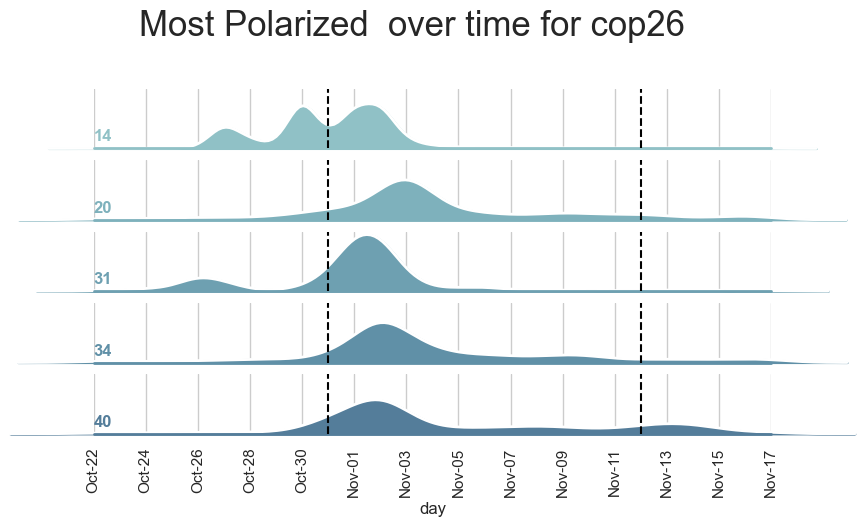
\includegraphics[width=0.75\linewidth]{Chapter5/figures/ridge_most_26.png}
     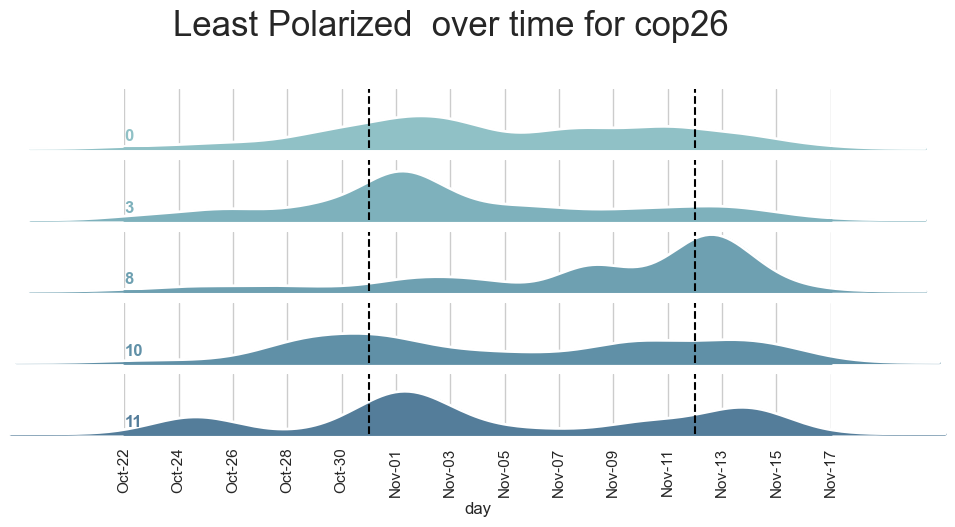
\includegraphics[width=0.75\linewidth]{Chapter5/figures/ridge_least_26.png}
    \caption{Enter Caption}
    \label{fig:ridge_topics}
\end{figure}


\section{RQ2 Longitudinal analysis}



\section{RQ3 User polarization among different topics}
After computing the polarization score for all users we can now analyze whether the the users are polarized in the same way among all the topics they were active in.

The number of users involved in this analysis is 22161 active in 26 topics. most of them (16141) were only active in one topic, the maximum is 23 and the average is 1.53 topics per user. 

Then we computed, for each user present in more than 1 topic, the average and the standard deviation of the score. This value is higher for the users that are present in both side of the spectrum so this allow us to identify the degree to which users tend to be monopolar.

Fig \ref{fig:std_avg} show how the distribution of the average score for every topic aggregated together, this matches with the global results of Falkenberg, where a majority is present on the $-1$ side versus a minority in the $1$ side.

In the std we can see how there is a strong tendency to stay in the same side of the spectrum.

\begin{figure}
    \centering
    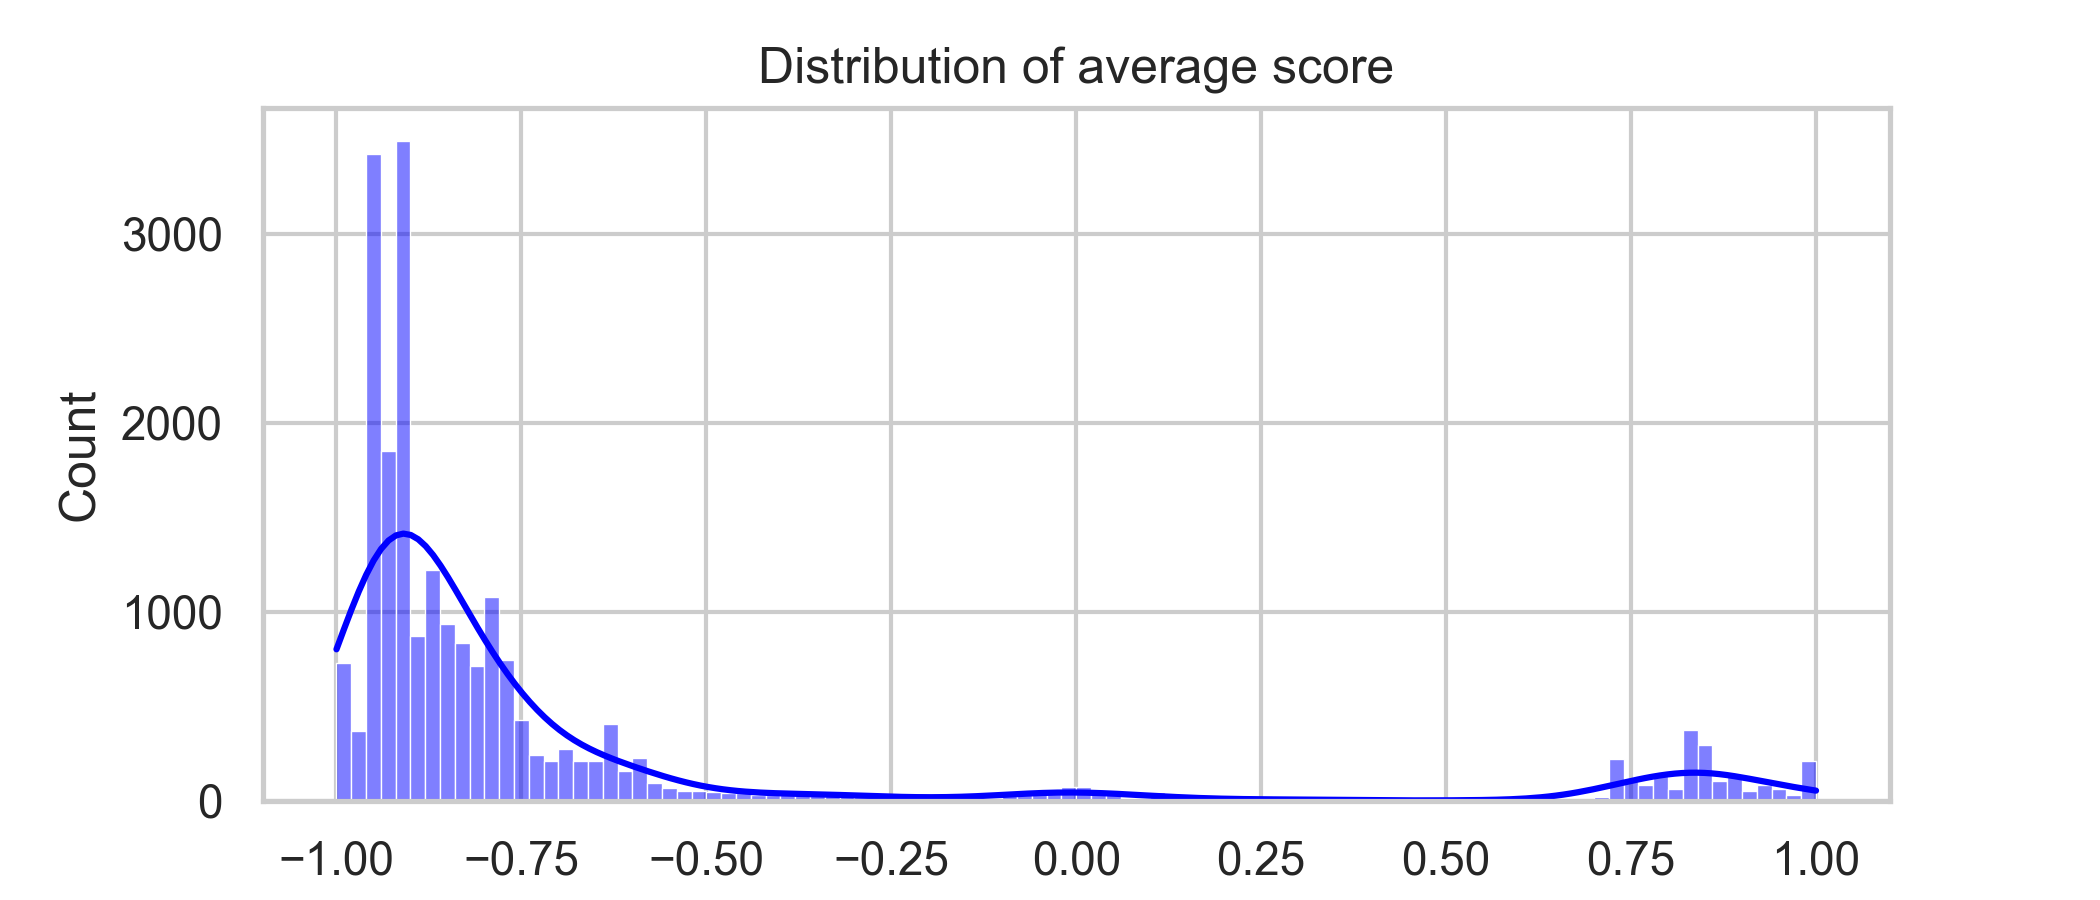
\includegraphics[width=0.9\linewidth]{Chapter5//figures/avg_score.png}
    
    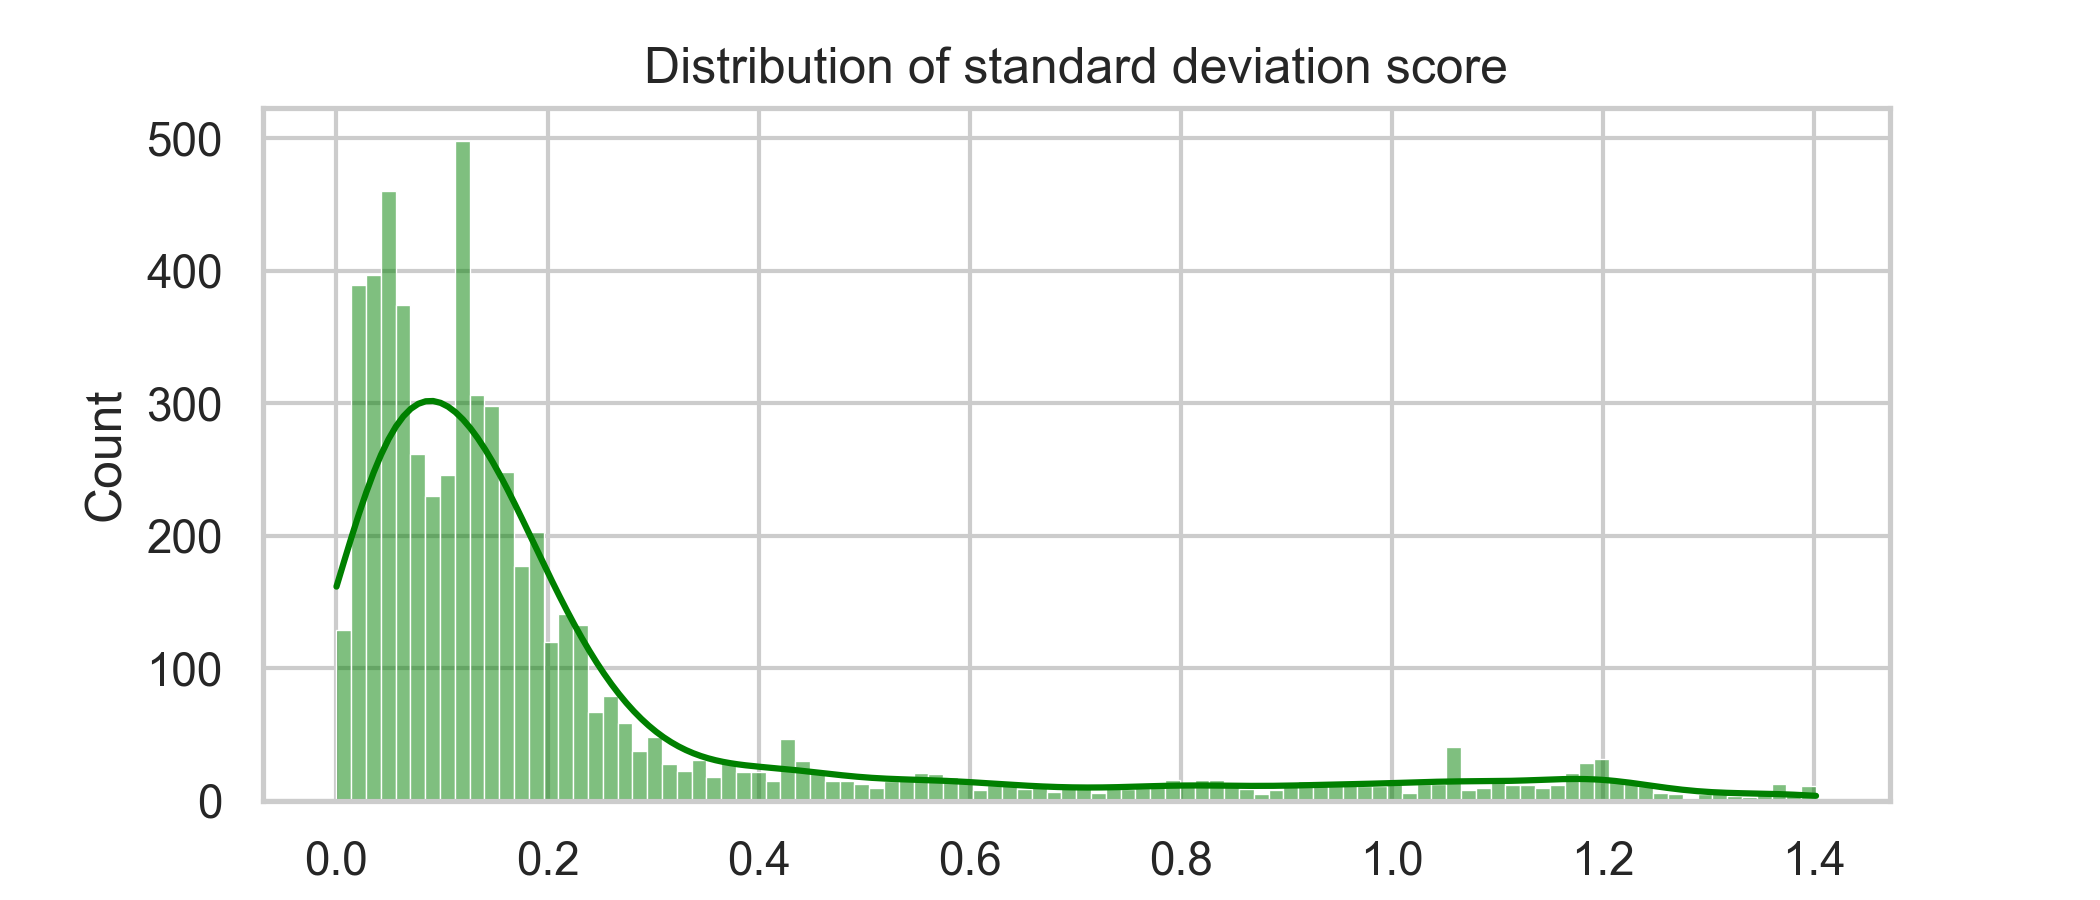
\includegraphics[width=0.9\linewidth]{Chapter5//figures/std_score.png}
    \caption{Enter Caption}
    \label{fig:std_avg}
\end{figure}



\section{RQ4 Polarization of experts vs know-it-all }
